\tikzstyle{webcam} = [rectangle, minimum width=6cm, minimum height=1cm, text centered, text width=6cm, draw=black, fill=black!10]
\tikzstyle{rasppi} = [rectangle, minimum width=1.5cm, minimum height=1cm, text centered, text width=3.5cm, draw=black, fill=black!10]
\tikzstyle{monattnd} = [rectangle, minimum width=1.5cm, minimum height=1cm, text centered, text width=3.5cm, draw=black, fill=black!10]
\tikzstyle{storeres} = [rectangle, minimum width=6cm, minimum height=1cm, text centered, text width=6cm, draw=black, fill=black!10]
\tikzstyle{arrow} = [thick,->,>=stealth]
\begin{figure}[h!]
	\begin{center}
		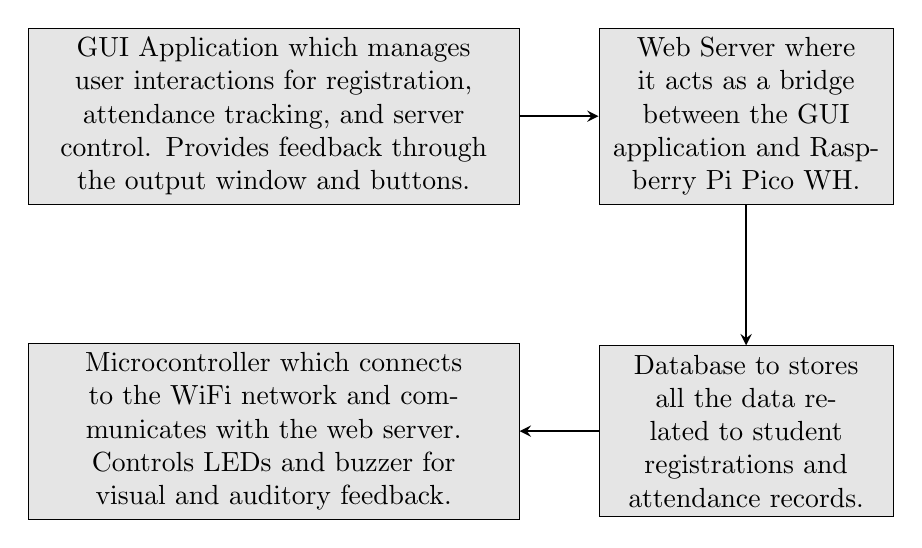
\begin{tikzpicture}[node distance=2cm]
			\node (WC) [webcam] {GUI Application which manages user interactions for registration, attendance tracking, and server control. Provides feedback through the output window and buttons.};
			\node (RP) [rasppi, right of=WC, xshift=4cm] {Web Server where it acts as a bridge between the GUI application and Raspberry Pi Pico WH.};
			\node (MA) [monattnd, below of=RP, yshift=-2cm] {Database to stores all the data related to student registrations and attendance records.};
			\node (SR) [storeres, left of=MA, xshift=-4cm] {Microcontroller which connects to the WiFi network and communicates with the web server. Controls LEDs and buzzer for visual and auditory feedback.};

			\draw [arrow] (WC) -- (RP);
			\draw [arrow] (RP) -- (MA);
			\draw [arrow] (MA) -- (SR);
		\end{tikzpicture}
	\end{center}
	\caption{Block Diagram}
\end{figure}
